\documentclass[a4paper,11pt]{article}
\usepackage[margin=25mm,headheight=16pt,headsep=8pt]{geometry}
\usepackage[T1]{fontenc}
\usepackage[utf8]{inputenc}
\usepackage{lmodern}
\usepackage[french]{babel}
\usepackage{graphicx,booktabs,tabularx,array,enumitem,xcolor,tikz}
\usepackage{fancyhdr}
\usepackage[hidelinks]{hyperref}
\graphicspath{{figures/}}
\definecolor{reportblue}{HTML}{163A5F}
\definecolor{reportgray}{HTML}{5D6875}
\setlength{\parindent}{0pt}
\setlength{\parskip}{6pt}
\setlist{nosep,leftmargin=*}
\providecommand{\NoAutoSpacing}{}
\newcommand{\reportmeta}[2]{\textcolor{reportgray}{\scriptsize #1}\par\textbf{#2}\par}
\newcommand{\film}[1]{\mbox{\NoAutoSpacing #1}}
\newcommand{\varname}[1]{\texttt{#1}}
\hypersetup{
  pdftitle={MCU --- Analyse des performances commerciales et critiques},
  pdfauthor={Lumu Bamana Manassé},
  pdflang={fr}
}
\pagestyle{fancy}
\fancyhf{}
\fancyhead[R]{\color{reportgray}\small Lumu Bamana Manassé}
\fancyfoot[C]{\thepage}
\renewcommand{\headrulewidth}{0.4pt}
\renewcommand{\footrulewidth}{0pt}
\renewcommand{\headrule}{{\color{reportblue}\hrule width\headwidth height\headrulewidth}}

\begin{document}
\begin{titlepage}
  \begin{tikzpicture}[remember picture,overlay]
    \fill[reportblue] (current page.north west) rectangle
      ([yshift=-42mm]current page.north east);
    \fill[reportblue!15] ([yshift=-42mm]current page.north west) rectangle
      ([yshift=-47mm]current page.north east);
  \end{tikzpicture}
  \vspace*{18mm}
  {\color{white}\sffamily\Large PROJET DATA ANALYTICS}\par
  \vspace{25mm}
  {\color{reportblue}\sffamily\fontsize{27}{32}\selectfont\bfseries
    MCU --- Analyse des performances commerciales et critiques\par}
  \vspace{5mm}
  {\large Analyse des films du Marvel Cinematic Universe --- Phases 1 à 5\par}
  \vspace{8mm}
  {\large Période analysée : 2008--2024\par}
  \vspace{12mm}
  {\sffamily\large\bfseries\color{reportblue} Lumu Bamana Manassé --- Data Analyst\par}
  \vspace{2mm}
  {\sffamily\large MediJr\par}
  \vspace{2mm}
  {\sffamily\small\color{reportgray}%
    GitHub : MediJr ---
    \href{https://github.com/MediJr}{\textcolor{reportblue}{\nolinkurl{https://github.com/MediJr}}}\par}
  \vfill
  \begin{tabular}{@{}ll@{}}
    \reportmeta{Projet}{Data Analytics} &
    \reportmeta{Période}{2008--2024}\\[7mm]
    \reportmeta{Périmètre}{Phases 1 à 5} &
    \reportmeta{Date}{septembre 2026}
  \end{tabular}
  \vfill
\end{titlepage}

\tableofcontents
\newpage

\section{Synthèse exécutive}

\subsection{Contexte}

L'objectif de cette analyse est d'étudier les performances commerciales et
critiques des films du Marvel Cinematic Universe (MCU), afin de mieux
comprendre les tendances observées au sein du catalogue et les facteurs
associés aux performances des films.

L'analyse porte sur 34 films couvrant les Phases 1 à 5 du MCU, avec des
informations relatives aux dates de sortie, budgets de production, recettes
au box-office, bénéfices calculés, retour sur investissement (ROI) ainsi
qu'aux évaluations critiques et spectateurs.

\subsection{Principaux résultats}

Sur l'ensemble du dataset, les films représentent un budget de production
cumulé de 6~947 millions de dollars et un box-office mondial cumulé de
31~129 millions de dollars.

Le bénéfice calculé selon la définition retenue dans le dataset, soit :
\begin{center}
\textbf{Profit = Box-office mondial $-$ Budget de production}
\end{center}
atteint 24~182 millions de dollars.

La note IMDb moyenne du catalogue est de 7,26/10.

L'analyse par phase met en évidence des différences importantes. La Phase~3
présente le box-office moyen, le profit moyen et le ROI global les plus
élevés dans le dataset étudié. À l'inverse, les indicateurs financiers moyens
observés en Phase~5 sont plus faibles que ceux des phases précédentes.

L'analyse des relations entre variables montre également une association
positive entre le budget de production et le box-office mondial. Une
association positive est également observée entre la note IMDb et le
box-office mondial.

Ces relations doivent toutefois être interprétées comme des associations
statistiques et non comme des relations de causalité.

\section{Objectifs de l'analyse}

L'analyse répond au brief métier suivant :

\begin{quote}
\og Nous souhaitons analyser les performances commerciales et critiques des
films du Marvel Cinematic Universe afin de mieux comprendre les facteurs
associés au succès d'un film.

Nous voulons notamment comparer les performances entre les différentes
phases du MCU, étudier la relation entre les investissements et les recettes,
analyser la rentabilité des films et comparer leurs performances critiques.

À partir de cette analyse, nous souhaitons obtenir des indicateurs et des
visualisations permettant à la direction de mieux comprendre les tendances
de performance du catalogue. \fg
\end{quote}

À partir de ce besoin, plusieurs axes d'analyse ont été retenus :
\begin{itemize}
  \item mesurer la performance commerciale ;
  \item comparer les différentes phases du MCU ;
  \item analyser la relation entre investissement et recettes ;
  \item mesurer la rentabilité ;
  \item comparer les performances critiques ;
  \item rechercher des facteurs associés aux performances commerciales ;
  \item observer l'évolution des performances dans le temps.
\end{itemize}

\section{Données et périmètre}

\subsection{Source des données}

Le dataset utilisé contient 34 films du MCU couvrant la période 2008--2024
et comprend 20 variables décrivant notamment les informations temporelles,
commerciales, financières et critiques des films.

Les principales sources mentionnées dans la documentation du dataset sont :
\begin{itemize}
  \item IMDb ;
  \item Box Office Mojo ;
  \item Rotten Tomatoes ;
  \item Wikipedia.
\end{itemize}

\subsection{Principales variables}

Les variables utilisées dans l'analyse comprennent notamment :
\begin{itemize}
  \item titre du film ;
  \item date et année de sortie ;
  \item phase du MCU ;
  \item ordre chronologique ;
  \item réalisateur ;
  \item acteur principal ;
  \item durée ;
  \item budget de production ;
  \item box-office mondial ;
  \item box-office domestique ;
  \item profit ;
  \item ROI ;
  \item part du box-office domestique ;
  \item note IMDb ;
  \item score Rotten Tomatoes ;
  \item score Metacritic.
\end{itemize}

Le dataset définit le profit comme la différence entre le box-office mondial
et le budget de production, tandis que le ROI correspond au rendement calculé
à partir du profit et du budget de production.

\section{Préparation et qualité des données}

\subsection{Profilage initial}

Un profilage technique du dataset a été réalisé avant l'analyse.

Les contrôles ont permis de confirmer :
\begin{itemize}
  \item 34 lignes et 20 colonnes ;
  \item aucune valeur manquante ;
  \item aucun doublon ;
  \item 34 identifiants de films uniques ;
  \item aucune incohérence entre phase et \varname{phase\_number} ;
  \item aucune incohérence entre \varname{release\_date} et
        \varname{release\_year} ;
  \item aucune valeur critique hors des intervalles attendus ;
  \item aucune durée négative.
\end{itemize}

\subsection{Contrôles de cohérence}

Des contrôles supplémentaires ont été effectués sur les variables calculées.

Les valeurs de :
\begin{itemize}
  \item \varname{profit\_millions} ;
  \item \varname{domestic\_percentage} ;
  \item \varname{roi\_percentage}
\end{itemize}
ont été comparées à leurs formules de calcul respectives.

Aucune incohérence n'a été détectée.

\subsection{Nettoyage}

La principale correction identifiée concernait le type de données de
\varname{release\_date}, initialement stocké comme texte.

La colonne a été convertie en véritable type date avant l'export du dataset
nettoyé.

Le fichier nettoyé a ensuite été utilisé pour la modélisation et l'analyse
dans Power BI.

\textbf{Conclusion sur la qualité :} les contrôles réalisés indiquent que le
dataset est cohérent et exploitable pour l'analyse retenue, avec une
correction de typage concernant la date de sortie.

\section{Méthodologie et architecture analytique}

L'analyse a été réalisée en plusieurs étapes :

\begin{tabularx}{\linewidth}{@{}
  >{\centering\arraybackslash}p{14mm}
  >{\raggedright\arraybackslash}p{46mm}
  X
  @{}}
  \toprule
  \textbf{Étape} & \textbf{Phase} & \textbf{Description} \\
  \midrule
  1 & Données brutes & Point de départ : données du dataset MCU \\
  2 & Profilage & Analyse de la structure, des types, des valeurs
      manquantes, des doublons et des distributions \\
  3 & Contrôle de qualité & Vérification de la validité, de la cohérence
      et de l'intégrité des données \\
  4 & Nettoyage & Correction des types et préparation du fichier
      exploitable \\
  5 & Analyse exploratoire & Exploration des données avec Python/Pandas
      et identification des principaux résultats \\
  6 & Modélisation & Construction du modèle en étoile dans Power BI \\
  7 & Indicateurs & Création des mesures analytiques avec DAX \\
  8 & Visualisation et analyse & Construction du tableau de bord et
      interprétation des résultats \\
  \bottomrule
\end{tabularx}

La modélisation Power BI repose sur un schéma en étoile comprenant :
\begin{itemize}
  \item \varname{Fact\_Movie} ;
  \item \varname{Dim\_Movie} ;
  \item \varname{Dim\_Phase} ;
  \item \varname{Dim\_Date}.
\end{itemize}

La granularité de la table de faits est :

\begin{center}
\textbf{1 film = 1 ligne dans \varname{Fact\_Movie}.}
\end{center}

Cette structure permet notamment d'analyser les performances selon le film,
la phase et la période de sortie.

\section{Analyse des résultats}

\subsection{Vue globale du catalogue}

Les principaux indicateurs du catalogue sont les suivants :

\begin{tabularx}{\linewidth}{@{}X r@{}}
  \toprule
  \textbf{Indicateur} & \textbf{Résultat} \\
  \midrule
  Nombre de films & 34 \\
  Budget total & 6~947~M\$ \\
  Box-office mondial total & 31~129~M\$ \\
  Profit calculé total & 24~182~M\$ \\
  Box-office mondial moyen & 915,56~M\$ \\
  Budget moyen & 204,32~M\$ \\
  ROI moyen par film & 339,58~\% \\
  Note IMDb moyenne & 7,26/10 \\
  Rotten Tomatoes moyen & 80,71~\% \\
  Metacritic moyen & 66/100 \\
  \bottomrule
\end{tabularx}

\begin{figure}[ht]
  \centering
  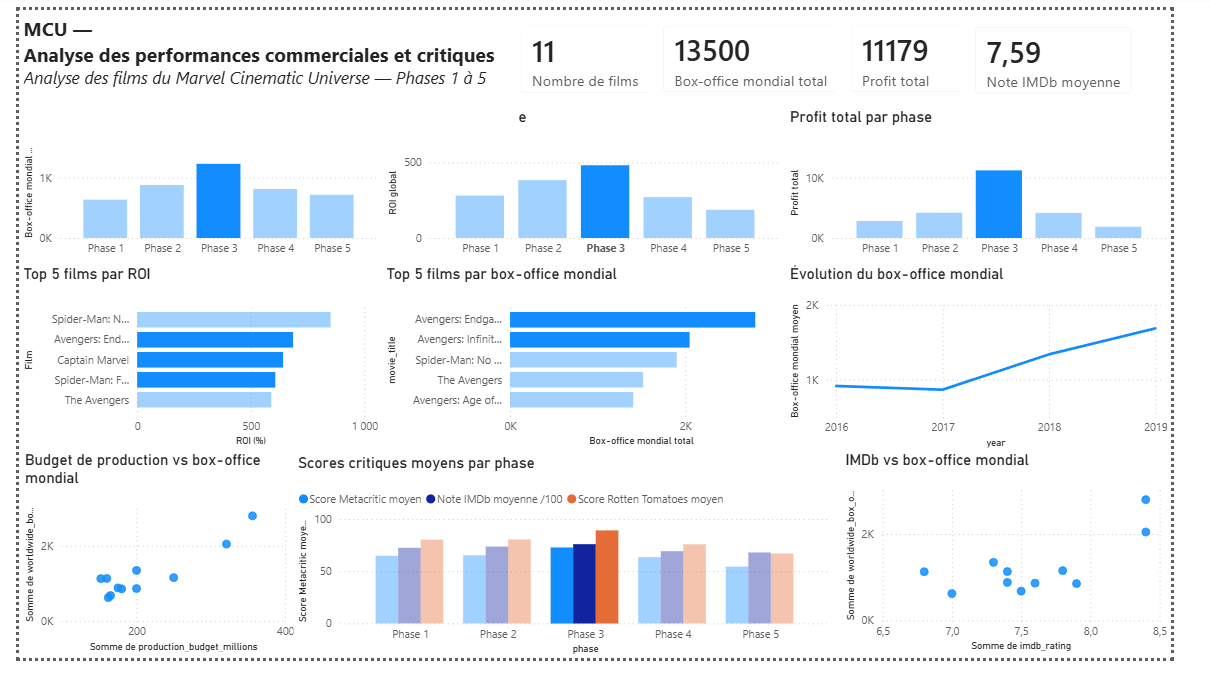
\includegraphics[width=\linewidth,keepaspectratio]{01_dashboard_global.png}
  \caption{Dashboard global MCU}
  \label{fig:dashboard-global}
\end{figure}

\subsection{Performance commerciale par phase}

Le box-office mondial moyen varie sensiblement selon les phases.

Les moyennes observées sont :

\begin{tabularx}{\linewidth}{@{}X r@{}}
  \toprule
  \textbf{Phase} & \textbf{Box-office mondial moyen} \\
  \midrule
  Phase 1 & 634,83~M\$ \\
  Phase 2 & 877,67~M\$ \\
  Phase 3 & 1~227,27~M\$ \\
  Phase 4 & 812,71~M\$ \\
  Phase 5 & 716,25~M\$ \\
  \bottomrule
\end{tabularx}

La Phase~3 présente donc le niveau moyen de box-office mondial le plus élevé
dans le périmètre étudié.

\begin{figure}[ht]
  \centering
  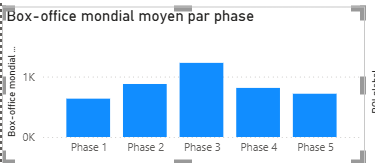
\includegraphics[width=\linewidth,keepaspectratio]{02_boxoffice_phase.png}
  \caption{Box-office mondial moyen par phase}
  \label{fig:boxoffice-phase}
\end{figure}

\subsection{Films générant les plus importants box-offices}

Les cinq films ayant généré les plus importants box-offices mondiaux dans le
dataset sont :

\begin{tabularx}{\linewidth}{@{}X r@{}}
  \toprule
  \textbf{Film} & \textbf{Box-office mondial} \\
  \midrule
  \film{Avengers: Endgame} & 2~798~M\$ \\
  \film{Avengers: Infinity War} & 2~048~M\$ \\
  \film{Spider-Man: No Way Home} & 1~902~M\$ \\
  The Avengers & 1~518~M\$ \\
  \film{Avengers: Age of Ultron} & 1~405~M\$ \\
  \bottomrule
\end{tabularx}

Ces résultats montrent que certains films contribuent fortement à la
performance commerciale globale du catalogue.

\begin{figure}[ht]
  \centering
  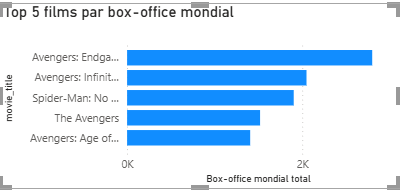
\includegraphics[width=\linewidth,keepaspectratio]{03_top5_boxoffice.png}
  \caption{Top 5 films par box-office mondial}
  \label{fig:top5-boxoffice}
\end{figure}

\subsection{Évolution du box-office dans le temps}

L'évolution annuelle fait apparaître des variations importantes de la
performance commerciale moyenne au cours de la période étudiée.

Les niveaux les plus élevés sont notamment observés autour de 2018--2019,
avec une nouvelle progression en 2024 dans le dataset.

L'évolution n'est donc pas linéaire : plusieurs périodes de progression et
de baisse sont observées.

\begin{figure}[ht]
  \centering
  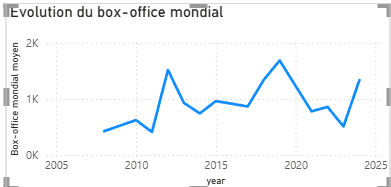
\includegraphics[width=\linewidth,keepaspectratio]{04_evolution_boxoffice.png}
  \caption{Évolution du box-office mondial}
  \label{fig:evolution-boxoffice}
\end{figure}

\subsection{Rentabilité et retour sur investissement}

Le ROI global a été calculé selon la formule :
\begin{center}
\textbf{ROI global = Profit total / Budget total $\times$ 100}
\end{center}

Cette méthode permet de mesurer l'efficacité globale des investissements
plutôt que de calculer simplement la moyenne des ROI individuels.

Les résultats par phase sont :

\begin{tabularx}{\linewidth}{@{}X r@{}}
  \toprule
  \textbf{Phase} & \textbf{ROI global} \\
  \midrule
  Phase 1 & 259,83~\% \\
  Phase 2 & 370,00~\% \\
  Phase 3 & 464,57~\% \\
  Phase 4 & 278,85~\% \\
  Phase 5 & 176,10~\% \\
  \bottomrule
\end{tabularx}

La Phase~3 présente ainsi le ROI global le plus élevé parmi les cinq phases
étudiées.

\begin{figure}[ht]
  \centering
  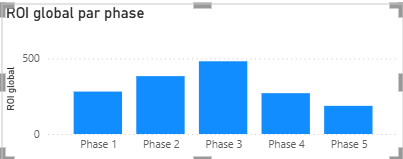
\includegraphics[width=\linewidth,keepaspectratio]{05_roi_phase.png}
  \caption{ROI global par phase}
  \label{fig:roi-phase}
\end{figure}

\subsection{Relation entre budget et box-office}

L'analyse du budget de production et du box-office mondial montre une
corrélation positive d'environ 0,63 dans le dataset.

Cela indique qu'au sein des données étudiées, les films bénéficiant de
budgets plus élevés tendent également à être associés à des box-offices plus
élevés.

Cependant, cette relation ne permet pas d'établir que l'augmentation du
budget provoque automatiquement une augmentation du box-office.

D'autres facteurs peuvent intervenir et ne sont pas directement mesurés dans
le dataset.

\begin{figure}[ht]
  \centering
  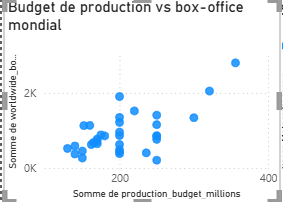
\includegraphics[width=\linewidth,keepaspectratio]{06_budget_boxoffice.png}
  \caption{Budget de production vs box-office mondial}
  \label{fig:budget-boxoffice}
\end{figure}

\subsection{Films présentant les ROI les plus élevés}

L'analyse du ROI individuel permet d'identifier les films ayant généré le
rendement le plus élevé par rapport à leur budget de production.

Les principaux résultats comprennent notamment :
\begin{itemize}
  \item \film{Spider-Man: No Way Home} ;
  \item \film{Avengers: Endgame} ;
  \item Captain Marvel ;
  \item \film{Spider-Man: Far From Home} ;
  \item The Avengers.
\end{itemize}

Le ROI constitue ici un indicateur complémentaire au box-office : un film
générant moins de recettes peut présenter un rendement supérieur s'il a été
produit avec un investissement relativement faible.

\begin{figure}[ht]
  \centering
  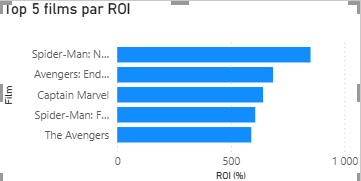
\includegraphics[width=\linewidth,keepaspectratio]{07_top5_roi.png}
  \caption{Top 5 films par ROI}
  \label{fig:top5-roi}
\end{figure}

\subsection{Profit par phase}

Le profit total varie également fortement entre les phases.

Les résultats montrent une contribution particulièrement importante de la
Phase~3, qui génère le profit total le plus élevé dans le dataset.

Cette observation est cohérente avec son niveau élevé de box-office et de ROI
global.

\begin{figure}[ht]
  \centering
  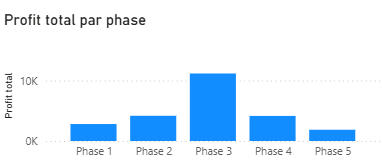
\includegraphics[width=\linewidth,keepaspectratio]{08_profit_phase.png}
  \caption{Profit total par phase}
  \label{fig:profit-phase}
\end{figure}

\subsection{Performance critique}

Trois indicateurs critiques ont été comparés :
\begin{itemize}
  \item IMDb ;
  \item Rotten Tomatoes ;
  \item Metacritic.
\end{itemize}

Pour faciliter la comparaison visuelle, la note IMDb a été convertie sur une
échelle de 100 pour cette visualisation uniquement.

Les moyennes observées par phase sont :

\begin{tabularx}{\linewidth}{@{}X rrr@{}}
  \toprule
  \textbf{Phase} & \textbf{IMDb /100} & \textbf{Rotten Tomatoes} &
  \textbf{Metacritic} \\
  \midrule
  Phase 1 & 72,5 & 80,33 & 64,83 \\
  Phase 2 & 73,7 & 80,50 & 65,33 \\
  Phase 3 & 75,9 & 89,09 & 72,73 \\
  Phase 4 & 69,3 & 75,86 & 63,57 \\
  Phase 5 & 68,0 & 67,00 & 54,50 \\
  \bottomrule
\end{tabularx}

Dans le dataset étudié, la Phase~3 présente les moyennes critiques les plus
élevées pour les trois indicateurs.

\begin{figure}[ht]
  \centering
  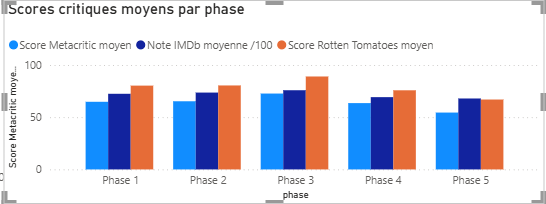
\includegraphics[width=\linewidth,keepaspectratio]{09_scores_critiques.png}
  \caption{Scores critiques moyens par phase}
  \label{fig:scores-critiques}
\end{figure}

\subsection{Réception critique et box-office}

L'analyse exploratoire montre une corrélation d'environ 0,66 entre la note
IMDb et le box-office mondial.

Cette relation est plus élevée que celles observées avec Rotten Tomatoes et
Metacritic :
\begin{itemize}
  \item IMDb $\leftrightarrow$ Box-office : 0,66
  \item Rotten Tomatoes $\leftrightarrow$ Box-office : 0,44
  \item Metacritic $\leftrightarrow$ Box-office : 0,42
\end{itemize}

Dans ce dataset, la note IMDb présente donc l'association statistique la plus
forte avec le box-office parmi les trois indicateurs critiques étudiés.

Il est toutefois important de rappeler qu'une corrélation ne démontre pas une
relation de causalité.

\begin{figure}[ht]
  \centering
  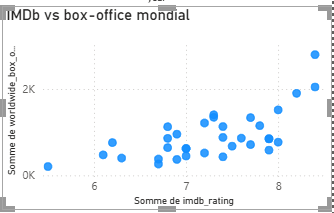
\includegraphics[width=\linewidth,keepaspectratio]{10_imdb_boxoffice.png}
  \caption{IMDb vs box-office mondial}
  \label{fig:imdb-boxoffice}
\end{figure}

\section{Conclusions}

L'analyse des 34 films étudiés met en évidence plusieurs enseignements.

\textbf{Premièrement,} les performances commerciales et financières varient
fortement selon les phases du MCU. La Phase~3 présente les niveaux moyens les
plus élevés de box-office ainsi que le ROI global et le profit total les plus
importants dans le périmètre étudié.

\textbf{Deuxièmement,} quelques films représentent une part importante des
performances commerciales du catalogue. \film{Avengers: Endgame},
\film{Avengers: Infinity War} et \film{Spider-Man: No Way Home} figurent
parmi les films générant les plus importants box-offices mondiaux.

\textbf{Troisièmement,} l'analyse met en évidence une association positive
entre le budget de production et le box-office mondial. Cependant, le budget
ne suffit pas à expliquer à lui seul les performances commerciales.

\textbf{Quatrièmement,} la réception critique présente également une
association positive avec le box-office, particulièrement dans le cas de la
note IMDb. Cette observation suggère qu'il peut être pertinent d'étudier
conjointement les indicateurs commerciaux et critiques.

\textbf{Enfin,} les résultats montrent une diminution des indicateurs moyens
de performance commerciale, de rentabilité et de réception critique entre
certaines phases récentes et la Phase~3. Cette évolution constitue un point
d'attention qui mériterait une analyse plus approfondie.

\section{Recommandations}

Les recommandations suivantes sont directement fondées sur les résultats
observés.

\subsection{Suivre conjointement performance commerciale et rentabilité}

Le box-office seul ne permet pas de mesurer l'efficacité d'un investissement.

Il est donc recommandé de suivre simultanément :
\begin{itemize}
  \item le budget ;
  \item le box-office ;
  \item le profit ;
  \item le ROI.
\end{itemize}

Cette approche permet de distinguer les films générant beaucoup de recettes
de ceux qui transforment efficacement leur investissement en bénéfices.

\subsection{Comparer systématiquement les performances entre phases}

Les écarts observés entre les phases montrent l'intérêt d'un suivi périodique
des indicateurs par période.

Un tableau de bord permettant de comparer chaque nouvelle phase aux phases
précédentes pourrait faciliter l'identification rapide des changements de
performance.

\subsection{Examiner les facteurs associés à la performance commerciale}

La relation observée entre budget et box-office ainsi que celle observée
entre IMDb et box-office justifient une analyse complémentaire des facteurs
associés au succès commercial.

Une analyse future pourrait intégrer d'autres variables telles que :
\begin{itemize}
  \item genre ;
  \item personnage principal ;
  \item réalisateur ;
  \item franchise ;
  \item calendrier de sortie ;
  \item marketing ;
  \item concurrence au moment de la sortie ;
  \item contexte économique ;
  \item durée d'exploitation.
\end{itemize}

Cela permettrait d'aller au-delà des variables actuellement disponibles.

\subsection{Porter une attention particulière aux performances des phases
récentes}

Les indicateurs moyens observés pour les phases 4 et 5 sont inférieurs à ceux
de la Phase~3 sur plusieurs dimensions.

Il serait donc pertinent de réaliser une analyse approfondie des films
concernés afin d'identifier les caractéristiques communes aux performances
les plus faibles et aux performances les plus élevées.

Cette analyse devrait distinguer les tendances générales des cas individuels
afin d'éviter de tirer des conclusions à partir d'un nombre limité de films.

\subsection{Mettre en place un suivi régulier des indicateurs}

Le dashboard Power BI peut servir de base à un système de suivi des
performances.

Les indicateurs principaux à suivre seraient notamment :

\textbf{Performance commerciale}
\begin{itemize}
  \item box-office mondial ;
  \item box-office moyen ;
  \item évolution temporelle.
\end{itemize}

\textbf{Rentabilité}
\begin{itemize}
  \item profit ;
  \item ROI ;
  \item budget.
\end{itemize}

\textbf{Performance critique}
\begin{itemize}
  \item IMDb ;
  \item Rotten Tomatoes ;
  \item Metacritic.
\end{itemize}

L'utilisation régulière de ces indicateurs permettrait de suivre l'évolution
du catalogue et de comparer les nouvelles productions aux performances
historiques.

\section{Limites de l'analyse}

Plusieurs limites doivent être prises en compte lors de l'interprétation des
résultats.

\subsection{Taille du dataset}

L'analyse porte sur seulement 34 films. Les résultats doivent donc être
interprétés dans le périmètre de ce dataset et ne doivent pas être
généralisés automatiquement à l'ensemble de l'industrie cinématographique.

\subsection{Définition du profit}

Le profit utilisé dans cette analyse correspond à :
\begin{center}
\textbf{Box-office mondial $-$ budget de production}
\end{center}

Il s'agit donc d'un indicateur calculé, et non nécessairement du bénéfice
comptable réel d'un studio.

Les coûts de marketing, distribution, taxes, commissions et autres dépenses
ne sont pas intégrés dans cette formule.

\subsection{Corrélation et causalité}

Les corrélations observées permettent d'identifier des associations entre
variables, mais elles ne permettent pas d'établir une causalité.

Par exemple, une corrélation positive entre budget et box-office ne signifie
pas nécessairement qu'un budget plus élevé entraîne directement davantage de
recettes.

\subsection{Variables non disponibles}

Certains facteurs susceptibles d'influencer les performances commerciales ne
figurent pas dans le dataset.

Les résultats doivent donc être considérés comme une analyse descriptive et
exploratoire du catalogue étudié.

\section{Outil de restitution}

Un dashboard Power BI interactif a été développé afin de permettre
l'exploration des résultats.

Le dashboard regroupe :
\begin{itemize}
  \item les KPI principaux ;
  \item la performance par phase ;
  \item les films les plus performants ;
  \item l'évolution temporelle ;
  \item le ROI ;
  \item le profit ;
  \item les scores critiques ;
  \item la relation budget/box-office ;
  \item la relation IMDb/box-office.
\end{itemize}

Les visualisations ont été sélectionnées à partir des besoins métier afin
d'éviter de multiplier les graphiques sans valeur analytique supplémentaire.
La sélection finale comprend 9 visualisations principales couvrant les
dimensions commerciales, financières, critiques et temporelles du problème.

\begin{figure}[ht]
  \centering
  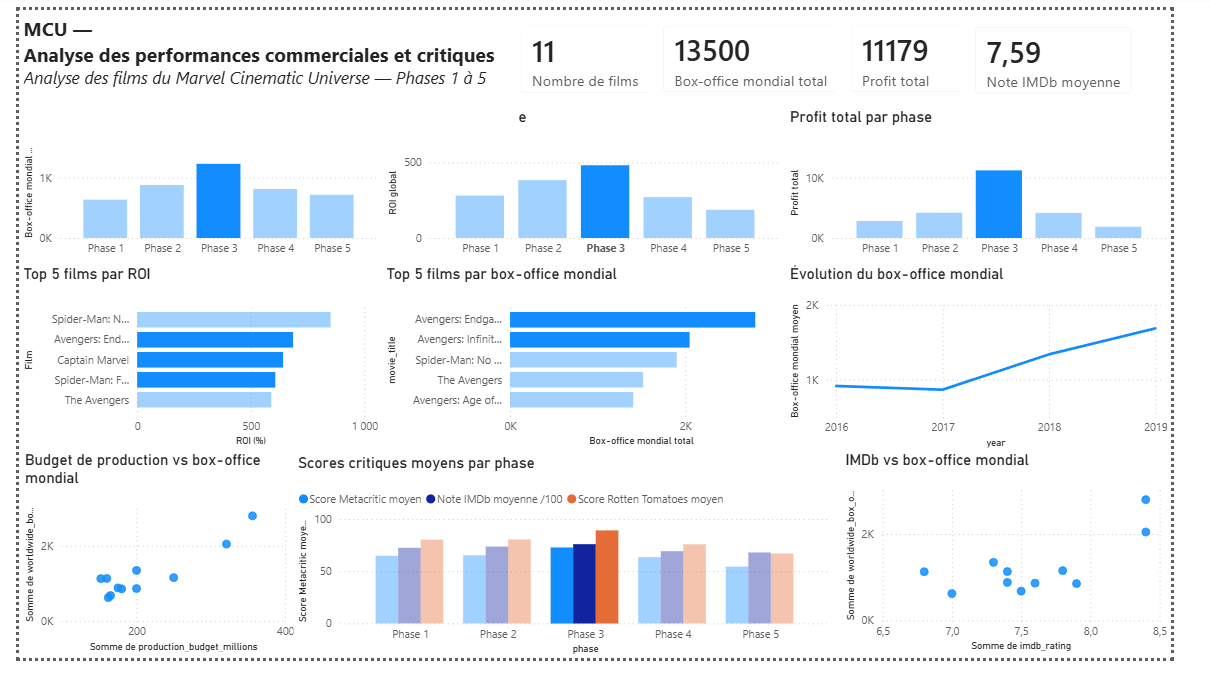
\includegraphics[width=\linewidth,keepaspectratio]{01_dashboard_global.png}
  \caption{Tableau de bord Power BI final}
  \label{fig:dashboard-final}
\end{figure}

\section{Conclusion finale}

Cette analyse a permis de construire une chaîne complète allant de la
compréhension du besoin métier jusqu'à la restitution interactive des
résultats.

Le projet a couvert :
\begin{itemize}
  \item le cadrage du problème ;
  \item l'inventaire et la compréhension des données ;
  \item le profilage ;
  \item le contrôle de qualité ;
  \item le nettoyage ;
  \item l'analyse exploratoire avec Python ;
  \item la modélisation dimensionnelle ;
  \item la création de mesures DAX ;
  \item la conception de visualisations adaptées aux questions métier ;
  \item la réalisation d'un dashboard Power BI interactif.
\end{itemize}

Les résultats permettent de mieux comprendre les différences de performance
entre les phases du MCU, la relation entre investissements et recettes, la
rentabilité des films et les associations entre réception critique et
performance commerciale.

Le dashboard constitue ainsi un outil de synthèse permettant d'explorer les
performances du catalogue, tandis que le présent rapport fournit le contexte,
les méthodes, les principaux résultats, les conclusions et les pistes
d'analyse complémentaires.

\section{Annexes}

\subsection{Annexe A --- Liste des visualisations}

\begin{tabularx}{\linewidth}{@{}c X@{}}
  \toprule
  \textbf{N$^{\circ}$} & \textbf{Visualisation} \\
  \midrule
  1 & Box-office mondial moyen par phase \\
  2 & Top 5 films par box-office mondial \\
  3 & Évolution du box-office mondial \\
  4 & ROI global par phase \\
  5 & Budget de production vs box-office mondial \\
  6 & Top 5 films par ROI \\
  7 & Profit total par phase \\
  8 & Scores critiques moyens par phase \\
  9 & IMDb vs box-office mondial \\
  \bottomrule
\end{tabularx}

Cette sélection correspond à la conception finale définie pour le dashboard.

\subsection{Annexe B --- Fichiers du projet}

Les principaux fichiers techniques du projet comprennent notamment :
\begin{itemize}
  \item dataset original ;
  \item dataset nettoyé ;
  \item scripts Python de profilage, nettoyage et analyse ;
  \item modèle Power BI ;
  \item rapport d'analyse.
\end{itemize}

\end{document}
